\documentclass{article}

\usepackage[margin=1in]{geometry}
\usepackage{amsmath, amssymb}
\usepackage{tikz}
\usepackage{enumitem}
\usepackage[T1]{fontenc}
\usepackage{hyperref}
\usepackage{amstext}
\hypersetup{
    colorlinks=true,
    linkcolor=blue,
    filecolor=blue,
    urlcolor=blue,
    }

\title{Deriving SLOs Equations}
\author{Jansel Valentin}
\date{}

\begin{document}
\maketitle

\begin{abstract}
\noindent Google provides SLO-related several equations without explaining how they derived them. This document shows how they are derived.
\end{abstract}

\section*{Context}

Imagine a system for which we define an SLO of 99.9\% ($S = 0.999$) over the last 30 days ($W$) and allowed error rate of $E = (1 - S) = 0.001$.

\quad

\noindent If this system has a 30 days throughput of $\mathrm{N}$, the \textbf{error budget} for this same period is $\mathrm{EB} \;=\; E \cdot N$

\section{Deriving Burn Rate}

If we were to consider a past performance of the system, say the previous month, we could compare the actual failure rate with the allowed monthly error rate and see how we did.

\[
\mathrm{burn\_rate_{30days}} \;=\; \frac{\mathrm{total\_failures}}{\mathrm{EB}}
\]
And we could say things such as: past month we burnt $2x$ or our error budget which means we burn twice as we were allowed too. Likewise, $0.9x$ would mean that we burn 90\% of what were allowed too.

\quad

\noindent But since we usually want to understand how the system is doing \emph{now} and whether the current performance will breach the SLO if left unchecked, we evaluate the system on a smaller window than the 30 days the SLO is defined on.

\quad

Let the short measurement window have duration $\Delta t$ (say \textbf{1 hour}), then \emph{throughput} in that hour

\[
q \;=\; \frac{N_{\Delta t}}{\Delta t} \;=\; \text{request/hour}
\]
and the bad events ($\mathrm{B}$) ratio in that same hour
\[
e_{\Delta t} \;=\; \frac{B_{\Delta t}}{N_{\Delta t}}
\]

Then I'd like to know what is the $\mathrm{EB_{\Delta t}}$ that my SLO allow me to consume in that $\Delta t$. We can do that by applying the same SLO variables because those definitions are not tied to the 30 days window.
\[
\mathrm{EB_{\Delta t}} \;=\; E \cdot N_{\Delta t}
\]
\emph{This is just ``Request'' not ``Request/hour''}

\quad

\noindent \textbf{Actual bad-event $\mathrm{B}$ rate in that hour}

\[
\lambda \;=\; \frac{B_{\Delta t}}{\Delta t} \;=\; \text{requests/hour}
\]
but note:
\[
\lambda \;=\; \frac{B_{\Delta t}}{\Delta t} \;=\; \frac{B_{\Delta t}}{N_{\Delta t}} \cdot \frac{N_{\Delta t}}{\Delta t} \;=\; e_{\Delta t} \cdot q
\]

\noindent \textbf{Allowed bad events rate (given by SLO)}

\[
\lambda_{\text{allowed}} \;=\; E \cdot q \;=\; \text{request/hour}
\]

\noindent Now if we compare how the \textbf{actual} error rate and the maximum \textbf{allowed} in that hour as per SLO
\[
\frac{\lambda}{\lambda_{\text{allowed}}} \;=\; \frac{e_{\Delta t} \cdot q}{E \cdot q} \;=\; \frac{e_{\Delta t}}{E} \;=\; \textbf{burn\_rate} \;=\; BR_{\Delta t}
\]

so the \textbf{burn rate} is understood as the \emph{actual} error rate in a chosen window divided by the allowed error rate $\mathrm{E}$ as per SLO definition.

\section{Deriving Time to Exhaust}

Say that conditions stay unchanged, then the time to burn the entire budget allocated for the entire window $\mathrm{W}$ is:
\[
t_{\text{exhaust}} \;=\; \frac{EB}{\lambda} \;=\; \frac{EB_{\text{requests}}}{\lambda_{request/hour}} \;=\ \frac{EB}{\lambda} \text{hours}
\]

\noindent But also notice that if we assume the system is stable and have the approximately same throughput $q$ over any hour, then the 30 days budget can be written as $EB = E \cdot (q \cdot W)$ and then

\[
t_{\text{exhaust}} \;=\; \frac{E \cdot (q \cdot W)}{\lambda} \;=\; \frac{E \cdot (q \cdot W)}{e_{\Delta t} \cdot q} \;=\; \frac{E \cdot W}{e_{\Delta t}} \;=\; \frac{E}{e_{\Delta t}} \cdot W \;=\; \frac{W}{BR_{\Delta t}}
\]

\section{Deriving Budget \% consumed by the time the alert fires}

\paragraph{From which we can know:}
``\textit{which burn rate do we need if we're willing to give up X\% of error budget in X period (1h)}''

\quad

\noindent Imagine a continium:

$$
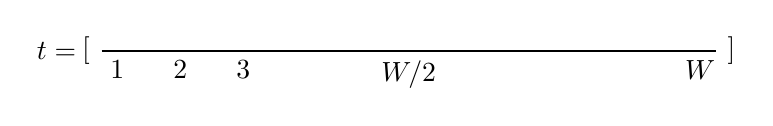
\begin{tikzpicture}[baseline=(current bounding box.center)]
    \node[left] at (0, 0) {$t=$};

    % axis with brackets
    \node at (0.0, 0) {$[$};
    \node at (8.2, 0) {$]$};

    %line inside
    \draw[thick] (0.2, 0) -- (8.0, 0);

    % labels
    \node[below] at (0.4, 0) {$1$};
    \node[below] at (1.2, 0) {$2$};
    \node[below] at (2.0, 0) {$3$};
    \node[below] at (4.1, 0) {$W/2$};
    \node[below] at (7.8, 0) {$W$};
\end{tikzpicture}
$$

\noindent For the 30 days we have $\texttt{budget\_per\_day} \;=\; \displaystyle \frac{\mathrm{EB}}{\mathrm{W}}$ and for each our \emph{t} we have $\texttt{burn\_rate\_t} \;=\; \displaystyle \frac{e_t}{E}$

\quad

\noindent Our burning rate indicates now many events per \emph{t} we're effectively consuming and is
a multiplier of what I am allowed to consume. E.g. If over $\mathrm{W = \text{30 days}}$ I'm allowed
to consume 90 events ($\mathrm{EB}$), then per day I'm meant to consume $\texttt{budget\_day} = 90/30 = \text{3 events}$.

\quad

If \textbf{burn\_rate = 2}, each day I'll be effectively consuming $2 * 3$ events. So $burn\_rate * budget\_day$ denotes my effective daily consumption.

\quad

at any point the \% of $\mathrm{EB}$ consumed at time $t$ is:

\begin{align*}
\%(t) & \;=\; \frac{t \cdot \mathrm{budget\_day} \cdot \mathrm{burn\_rate}}{\mathrm{EB}} \\
& \;=\; \frac{t \cdot \mathrm{(EB / W)} \cdot \mathrm{burn\_rate}}{\mathrm{EB}} \\
& \;=\; \frac{t \cdot \mathrm{burn\_rate}}{\mathrm{W}} \\
& \;=\; \frac{t}{W} \cdot \mathrm{burn\_rate}
\end{align*}

\subsection{Which burn rate do I need if I'm willing to give up 5\% of budget in 1h?}

Now, if over \emph{t = 1h} I'm willing to give up 5\% of the budget, I'll need a \textbf{burn\_rate} of

\[
\frac{5\% \cdot \mathrm{W} \quad \textit{(in hours)}}{t} \;=\; \mathrm{burn\_rate}
\]

replacing by $t = 1h$, $W = 720h$, give us a \textbf{burn\_rate} of 36

\section{Deriving Time Taken for an Alert to Fire}

\paragraph{Conditions to trigger alert:}
This section help us identify the conditions to trigger the alert. This needs to be considered alongside section 3.1 because the burn\_rate here is one we've chosen so that it guarantee us that no more than X\% of the entire budget is consumed. Let's say we've chosen burn\_rate to be 36 and that we're willing to give up 5\% of the entire budget in 1h

\quad

\noindent If we pick an aggregation window $T = 1h$ and we start observing an error rate \emph{r} (which naturally grows over time $t \in [0, T]$). If we assume that our error rate $r$ grows linearly with $t$ where $t < T$.

\quad

We define this error rate for the aggregated period T when evaluated at $t$ as

\[
\mathrm{error\_rate\_t} = r \cdot t/T
\]

so is a linear function $t$

\quad

We know that the maximum errors we can have in \textbf{T} overall is \textbf{E}, so:
\[
\mathrm{burn\_rate} \;=\; \frac{\mathrm{error\_rate\_T}}{\mathrm{E}}
\]

and
\[
\mathrm{error\_rate\_T} \;=\; \mathrm{burn\_rate} \cdot \mathrm{E}
\]

but $error\_rate\_t \in [1, T]$  is defined as function $t$ (our relative time), we want to trigger the alert when the \emph{growing} $\mathrm{error\_rate\_t}$ reaches our maximum allowed error rate. So we want to check if
\[
\mathrm{error\_rate\_t} \;=\; \mathrm{error\_rate\_T} \quad \Rightarrow \quad r \cdot t/T \;=\; \mathrm{burn\_rate} \cdot \mathrm{E}
\]

Or to be more lenient on the equality we can trigger the alert if
but if our maximum error allowed is \textbf{E}, then:

\[
r \cdot t/T \;>\; \mathrm{burn\_rate} \cdot \mathrm{E} \quad \Rightarrow \quad r \cdot t/T \;>\; \mathrm{burn\_rate} \cdot \mathrm{(1 - SLO)}
\]

and the time $t$ for \textbf{T} = 1h where the alert will be triggered is:
\[
t = \frac{1 - SLO}{r} \cdot T \cdot burn\_rate
\]

\subsection{Intuition about \emph{r}}

It’s important to talk about what $r$ represents when an alert is triggered. And how long do we have to ``reset time'': \href{https://sre.google/workbook/alerting-on-slos/#:~:text=Alerting%20Considerations}{Alerting Considerations}

\quad

Since $r = bad/good$

\quad

if we take it to the extreme we can define $r = 1.0$ signifying total outage. This simplifies reasoning because we can then use the equation to understand the time the alert will be triggered when the aggregation window is \textbf{T} = 1h and we picked a $\mathrm{burn\_rate} = 36$ (because we're willing to give up 5\% error budget in an hour). then

\begin{align*}
t & \;=\; \frac{1 - SLO}{r} \cdot T \cdot burn\_rate \\
& \;=\; (1  -SLO) \cdot T \cdot burn\_rate \\
& \;=\; 0.001 \cdot 1h \cdot 36 \\
& \;=\; 0.036\ h \\
& \;=\; 2.16\ min
\end{align*}

so our alert will be fired in the first \textbf{2.16 min} from the first error occurrence.

\quad

\paragraph{Reset time:}
Talking about ``reset time'': how long alerts will keep firing after the issue's been solved?.

\quad

\noindent Imagine that an alert is triggered and the issue is immediately mitigated. Then since our errors will still be in the \textbf{T} = 1h rolling window until they age out, we'll have:

\quad

$1h - 2.16\ \text{min} \;=\; \sim58\ \text{min}$ until the errors age out.

\section*{References}

\begin{itemize}
    \item Defining SLOs: \href{Defining SLOs}{https://sre.google/workbook/implementing-slos/}
    \item Alerting on SLOs: \href{Alerting on SLOs}{https://sre.google/workbook/alerting-on-slos/}
\end{itemize}

\end{document}
